\documentclass[11pt,a4paper]{article}

\usepackage{fontspec}
\setmainfont{Times New Roman}
\usepackage[russian]{babel}

\usepackage[left=20mm,right=15mm,top=15mm,bottom=15mm]{geometry}
\usepackage{amsmath,amssymb,amsfonts}
\usepackage{graphicx}
\usepackage{booktabs}
\usepackage{array}
\usepackage{caption}
\usepackage{hyperref}
\usepackage{microtype}
\usepackage{float}

\hypersetup{
    colorlinks=true,
    linkcolor=black,
    urlcolor=blue,
    citecolor=black
}

\setlength{\parindent}{1.25cm}
\setlength{\parskip}{0.15em}
\linespread{1.1}
\setlength{\abovedisplayskip}{3pt}
\setlength{\belowdisplayskip}{3pt}

\begin{document}

% -------------------------------------------------------------
% ТИТУЛЬНЫЙ ЛИСТ
% -------------------------------------------------------------
\begin{titlepage}
    \centering
    {\bfseries\large Белорусский государственный университет\par}
    {\bfseries\large Факультет прикладной математики и информатики\par}
    
    \vspace{6cm}
    {\Huge\bfseries ОТЧЁТ\par}
    \vspace{0.5cm}
    {\large по лабораторной работе №4 по компьютерной графике\par}
    \vspace{0.5cm}
    {\Large\bfseries Алгоритмы отсечения отрезков и многоугольников двумерным окном\par}
    
    \vspace{6cm}
    \begin{flushright}
        \large
        \textbf{Выполнил:}\\
        студент 4 группы 3 курса\\
        Дикан Д.~А.\\[1em]
        \textbf{Преподаватель:}\\
        старший преподаватель\\
        Соловей Сергей Сергеевич
    \end{flushright}
    
    \vfill
    {\large Минск, 2026\par}
\end{titlepage}

\newpage

% -------------------------------------------------------------
% СТРАНИЦА 2: ЦЕЛЬ И ТЕОРИЯ
% -------------------------------------------------------------
\section*{1. Цель работы}
Изучить базовые алгоритмы отсечения отрезков двумерной областью видимости: алгоритм деления отрезка пополам (метод средней точки) для прямоугольного окна и параметрический алгоритм Кируса--Бека для произвольного выпуклого многоугольника. Провести анализ их вычислительных характеристик и разработать веб-приложение для наглядной визуализации отсечения произвольных наборов отрезков.

\section*{2. Теоретические сведения}
\begin{enumerate}
    \item \textbf{Коды областей (Коэна--Сазерленда).} Для прямоугольного окна $[X_{\min}, X_{\max}] \times [Y_{\min}, Y_{\max}]$ каждой точке плоскости $(x, y)$ сопоставляется 4-битный код $(T, B, R, L)$, где биты вычисляются по условиям:
    \begin{equation}
        T = (y > Y_{\max}), \quad B = (y < Y_{\min}), \quad R = (x > X_{\max}), \quad L = (x < X_{\min}).
    \end{equation}
    Для отрезка с кодами концов $c_1$ и $c_2$ выполняются побитовые проверки:
    \begin{align}
        c_1 \mid c_2 = 0 &\implies \text{отрезок целиком виден (тривиально принят)}, \\
        c_1 \ \& \ c_2 \neq 0 &\implies \text{отрезок целиком невидим (тривиально отброшен)}.
    \end{align}
    Если оба условия не выполнились, отрезок требует расчета точек пересечения. При этом равенство $c_1 \ \& \ c_2 = 0$ не гарантирует видимость: отрезок может проходить мимо угла окна через две смежные внешние области.

    \item \textbf{Алгоритм деления отрезка пополам (средняя точка).} Позволяет определить границы видимой части отрезка методом двоичного поиска без деления на угловой коэффициент. На отрезке $[A, B]$ рассчитывается середина:
    \begin{equation}
        M = \frac{A + B}{2} = \left(\frac{x_A + x_B}{2}, \, \frac{y_A + y_B}{2}\right).
    \end{equation}
    В целочисленных координатах деление на 2 заменяется быстрым побитовым сдвигом вправо. Если $c(M) \ \& \ c(B) \neq 0$, то половина $[M, B]$ заведомо невидима, и поиск границы продолжается на $[A, M]$, иначе граница смещается в $M$. Процесс повторяется до достижения заданной точности:
    \begin{equation}
        n = \left\lceil \log_2 \left(\frac{L}{\varepsilon}\right) \right\rceil \text{ шагов, где } L \text{ --- длина отрезка, } \varepsilon \text{ --- точность.}
    \end{equation}
    После сходимости к границе выполняется обязательная проверка принадлежности найденной точки окну, что исключает отрезки, проходящие мимо угла.

    \item \textbf{Алгоритм Кируса--Бека.} Применяется к произвольному выпуклому $m$-угольнику с обходом вершин $V_0, \dots, V_{m-1}$ против часовой стрелки. Отрезок задается параметрически:
    \begin{equation}
        P(t) = P_1 + t \cdot D, \quad \text{где } D = P_2 - P_1, \quad t \in [0, 1].
    \end{equation}
    Внутренняя нормаль к ребру $e_i = V_i V_{i+1}$ равна:
    \begin{equation}
        N_i = \bigl(-(y_{i+1} - y_i), \, x_{i+1} - x_i\bigr).
    \end{equation}
    Параметр $t_i$ в точке пересечения прямой отрезка с ребром вычисляется как:
    \begin{equation}
        t_i = -\frac{N_i \cdot W_i}{N_i \cdot D}, \quad \text{где } W_i = P_1 - V_i.
    \end{equation}
    Обновление параметров входа и выхода из многоугольника:
    \begin{equation}
        \begin{cases}
            t_{\text{in}} = \max(t_{\text{in}}, t_i), & \text{если } N_i \cdot D > 0 \quad (\text{вход}), \\
            t_{\text{out}} = \min(t_{\text{out}}, t_i), & \text{если } N_i \cdot D < 0 \quad (\text{выход}).
        \end{cases}
    \end{equation}
    Если $N_i \cdot D = 0$, отрезок параллелен ребру: при $N_i \cdot W_i < 0$ он лежит снаружи и отбрасывается. Отрезок видим, если $t_{\text{in}} \le t_{\text{out}}$.
\end{enumerate}

\newpage

% -------------------------------------------------------------
% СТРАНИЦА 3: АРХИТЕКТУРА И ОТСЕЧЕНИЕ ПРЯМОУГОЛЬНЫМ ОКНОМ
% -------------------------------------------------------------
\section*{3. Архитектура и реализация приложения}
\begin{itemize}
    \item \textbf{Серверная часть (Python 3, Flask):} файл \texttt{processing.py} реализует алгоритмы средней точки и Кируса--Бека с обработкой граничных случаев, файл \texttt{main.py} предоставляет веб-интерфейс и API для загрузки файлов и запуска отсечения.
    \item \textbf{Клиентская часть (HTML5, Tailwind CSS, Canvas API):} интерактивная координатная плоскость с масштабированием, подсветка отсекающего окна и видимых частей линий, ручной ввод и загрузка тестовых файлов формата n / отрезки / окно.
\end{itemize}

\section*{4. Результаты работы}
На рисунке 1 представлена визуализация отсечения контрольного набора отрезков прямоугольным окном $[0, 20] \times [0, 20]$ алгоритмом деления пополам (методом средней точки). Алгоритм корректно выполняет предварительную классификацию по 4-битным кодам концов, отсекая тривиально невидимые линии и находя координаты границ для отрезков, пересекающих контур окна.

\begin{figure}[H]
    \centering
    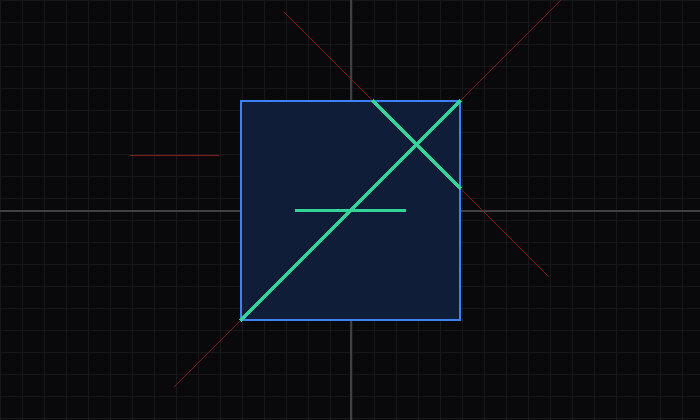
\includegraphics[width=0.72\textwidth]{../images/01_clipping_rect.png}
    \caption{Отсечение отрезков прямоугольным окном алгоритмом средней точки}
\end{figure}

\newpage

% -------------------------------------------------------------
% СТРАНИЦА 4: ОТСЕЧЕНИЕ МНОГОУГОЛЬНИКОМ И СРАВНЕНИЕ
% -------------------------------------------------------------
\section*{Отсечение произвольным выпуклым многоугольником}
На рисунке 2 представлена визуализация работы параметрического алгоритма Кируса--Бека на выпуклом шестиугольнике с вершинами $(-15, -10)$, $(0, -18)$, $(15, -10)$, $(15, 10)$, $(0, 18)$, $(-15, 10)$. Алгоритм корректно определяет входящие и выходящие точки пересечения и оставляет только видимые части отрезков (выделены зеленым цветом).

\begin{figure}[H]
    \centering
    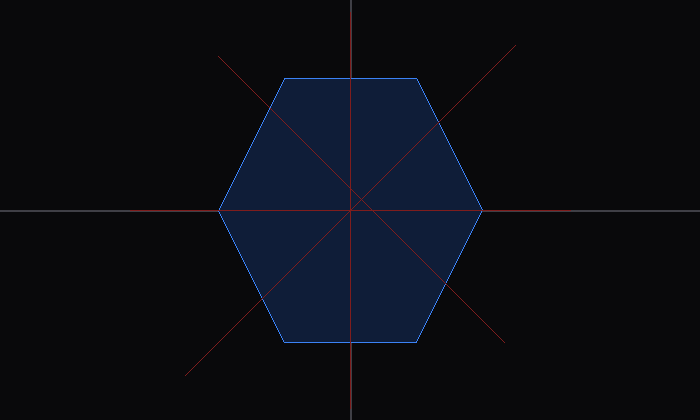
\includegraphics[width=0.68\textwidth]{../images/02_cyrus_beck_convex.png}
    \caption{Отсечение отрезков выпуклым шестиугольником алгоритмом Кируса--Бека}
\end{figure}

\section*{Сравнение характеристик алгоритмов}
В ходе практической проверки алгоритмов на контрольных данных и выборке из 1000 линий сопоставлены их вычислительные свойства:

\begin{table}[H]
\centering
\begin{tabular}{@{}p{3.8cm}>{\raggedright\arraybackslash}p{6.4cm}>{\raggedright\arraybackslash}p{6.4cm}@{}}
\toprule
\textbf{Характеристика} & \textbf{Алгоритм средней точки} & \textbf{Алгоритм Кируса--Бека} \\
\midrule
\textbf{Форма области} & Только прямоугольное окно с гранями, параллельными осям координат & Произвольный выпуклый $m$-угольник с обходом вершин против часовой стрелки \\
\textbf{Время (1000 линий)} & \textbf{3.54 мс} (в среднем $\approx 16$ шагов бисекции на отрезок) & \textbf{1.45 мс} (прямой расчет параметров $t$ для каждого ребра) \\
\textbf{Арифметика} & Сложение и побитовый сдвиг (деление на 2), без операции деления & Скалярные произведения векторов и вещественное деление \\
\textbf{Особые случаи} & Линии вне окна, но с $c_1 \ \& \ c_2 = 0$, требуют обязательной проверки точки & Параллельные отрезки ($N \cdot D = 0$) проверяются по знаку $N \cdot W$ \\
\bottomrule
\end{tabular}
\end{table}

\newpage

% -------------------------------------------------------------
% СТРАНИЦА 5: ВЫВОДЫ
% -------------------------------------------------------------
\section*{5. Выводы}
\begin{enumerate}
    \item \textbf{Коды областей ускоряют отсев.} Большинство отрезков сцены отсекается или принимается уже на этапе побитовых проверок, до любых вычислений координат пересечений. При этом нулевое побитовое И не гарантирует видимость~--- случай «мимо угла» требует дополнительной проверки, что подтверждено на контрольных примерах.
    \item \textbf{Бисекция медленнее прямого расчёта.} Алгоритм средней точки нашёл правильные пересечения во всех тестах, однако в среднем затратил $\sim$16 итераций на отрезок. Алгоритм Кируса--Бека даёт тот же результат за один проход, что и объясняет разницу во времени: 3.54 мс против 1.45 мс на 1000 отрезков.
    \item \textbf{Кирус--Бек работает с любым выпуклым многоугольником.} Параметрический подход не привязан к форме окна: достаточно задать нормали рёбер. Смена прямоугольника на шестиугольник не меняет структуру алгоритма, тогда как алгоритм средней точки потребовал бы полной переработки.
    \item \textbf{Невыпуклость ломает алгоритм.} Когда отрезок входит в область дважды, Кирус--Бек возвращает неверный интервал или ложно отбрасывает отрезок. Это прямое следствие предположения о единственном интервале $[t_{\text{in}}, t_{\text{out}}]$, которое перестаёт выполняться для невыпуклых контуров.
\end{enumerate}

\end{document}
